\documentclass[tikz,border=3mm]{standalone}
\usetikzlibrary{automata}

\begin{document}
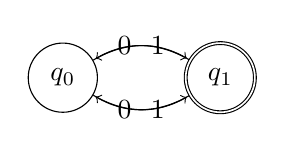
\begin{tikzpicture}[shorten >=1pt,node distance=2cm]
    % Nodes
    \node[state] (q_0) {$q_0$};
    \node[state,accepting] (q_1) [right of=q_0] {$q_1$};
    
    % Edges
    \draw[->] (q_0) edge[bend left] node[left] {0} (q_1);
    \draw[->] (q_0) edge[bend right] node[right] {1} (q_1);
    \draw[->] (q_1) edge[bend left] node[left] {0} (q_0);
    \draw[->] (q_1) edge[bend right] node[right] {1} (q_0);
\end{tikzpicture}
\end{document}